\documentclass[10pt,a4paper]{article}

\usepackage[T1]{fontenc}
\usepackage[utf8]{inputenc}
\usepackage{amsmath,amssymb,amsthm}
\usepackage{booktabs}
\usepackage{graphicx}
\usepackage[margin=1in]{geometry}
\IfFileExists{microtype.sty}{\usepackage{microtype}}{}
\usepackage{url}
\usepackage[hidelinks]{hyperref}

\theoremstyle{plain}
\newtheorem{theorem}{Theorem}[section]
\newtheorem{lemma}[theorem]{Lemma}
\newtheorem{proposition}[theorem]{Proposition}
\newtheorem{corollary}[theorem]{Corollary}
\theoremstyle{definition}
\newtheorem{definition}[theorem]{Definition}
\newtheorem{remark}[theorem]{Remark}
\newtheorem{example}[theorem]{Example}
\newtheorem{observation}[theorem]{Observation}

\newcommand{\NN}{\mathbb{N}}
\newcommand{\ZZ}{\mathbb{Z}}
\newcommand{\ind}{\alpha}
\newcommand{\forestnum}{f}
\newcommand{\bipnum}{b}
\newcommand{\treenum}{\mathrm{tree}}
\newcommand{\pathnum}{\mathrm{path}}
\newcommand{\de}{\mathrm{dist_{even}}}
\newcommand{\eh}{\mathrm{hor_{even}}}
\newcommand{\gt}{\gamma_t}
\newcommand{\gc}{\gamma_c}
\newcommand{\Ls}{L_s}
\newcommand{\blow}[2]{#1[K_{#2}]}

\title{The discretization cliff:\\
clique blow-ups of the $5$-cycle and a predictable failure mode\\
of database-verified conjecture generators}

\author{Kuber Mehta\thanks{Correspondence: \texttt{kuberwastaken@gmail.com}. All data, scripts and
certificates referenced here are in the public repository
\url{https://github.com/Kuberwastaken/c5-k4}; see Section~\ref{sec:repro}.}}

\date{Draft of \today}

\emergencystretch=3em
\hbadness=6000

\begin{document}
\maketitle

\begin{abstract}
Machine conjecture generators in the Graffiti lineage --- Fajtlowicz's \emph{Graffiti},
DeLaVi\~na's \emph{Graffiti.pc}, Larson and Van Cleemput's \emph{CONJECTURING}, Davila's
\emph{TxGraffiti} --- emit an inequality only after it has survived evaluation on a finite
stored database of graphs, and typically only if the database also contains a graph attaining
it with equality. We isolate a structural regime in which this filter is systematically
uninformative. On a clique blow-up $H[K_m]$, every ``induced-subgraph number'' associated with
a hereditary class of bipartite graphs --- the forest number $\forestnum$, the bipartite number
$\bipnum$, the induced-tree number $\treenum$, the induced-path number $\pathnum$ --- is
\emph{pinned}: it is bounded by $2\ind(H)$ for all $m$ and constant in $m$ for $m \ge 2$, while
$n$, $\Delta$, and the distance-, parity- and density-derived correction terms of the same
invariant vocabulary grow with $m$. Any conjectured lower bound on a pinned invariant by a
growing term therefore fails for all large $m$, and whenever the growing term lands exactly on
the pinned value, the last member on which the bound survives does so with \emph{equality}.

We work this out completely for $H = C_5$. For every $m \ge 1$ we prove
$\ind(\blow{C_5}{m}) = 2$ and $\pathnum = \treenum = \forestnum = \bipnum = 4$, and we give
closed forms for the growing side ($\Delta = 3m-1$, $\de = 2m+1$, $\eh = m(2m-1)$,
$n \bmod \Delta = 2m+1$ for $m \ge 3$). Four conjectures of \emph{Written on the Wall II} that
were open in July 2026 --- numbers $63$, $85$, $64$ and $309$ --- are then refuted by the family
with exact thresholds: all three of $63$, $85$, $64$ are attained with equality at $m = 3$
(order $15$) and violated for every $m \ge 4$; $309$ is attained with equality at $m = 1$ and
violated for every $m \ge 3$. An exhaustive evaluation of all $522$ transcribed WOWII records
against $\blow{C_5}{4}$ locates the same mechanism eight more times among conjectures already
refuted by others, and --- the larger half of the data --- exhibits the family as a zero-slack
witness for roughly three dozen further statements, including $19$ theorems of the corpus.
We state explicitly what this does \emph{not} establish: it is a mechanism and a diagnostic,
not a counterexample engine, and we make no claim here that tightness data can be navigated
prospectively.
\end{abstract}

\section{Introduction}

\subsection{Database-verified conjecture generation}

A conjecture generator of the Graffiti type maintains a finite collection of graphs
$\mathcal{D}$ together with precomputed values of a fixed vocabulary of invariants, forms
candidate inequalities between algebraic expressions in that vocabulary, and discards every
candidate falsified by some member of $\mathcal{D}$
\cite{fajtlowicz1988,delavina2005gpc,delavina2005history,larson2005survey,larsonvancleemput2016,davila2026txgraffiti}.
Surviving candidates are further filtered by significance heuristics; in Fajtlowicz's design and
its descendants the dominant heuristic (the ``Dalmatian'' rule and its variants) prefers bounds
that are \emph{attained} on $\mathcal{D}$ and that are not dominated by an already-retained bound
\cite{larsonvancleemput2016}. The output is thus, by construction, a set of statements that are
true on $\mathcal{D}$ and sharp on $\mathcal{D}$.

This is a strong filter, and the record of the programs shows it works: many Graffiti and
Graffiti.pc conjectures have become theorems, and DeLaVi\~na's \emph{Written on the Wall II}
(WOWII) list \cite{wowii} remains an actively worked source of open problems two decades after
its first entries. But the filter has an exact blind spot, and the blind spot is not random.
It is the set of graph families along which some invariants of the vocabulary are
\emph{constant} while others are \emph{unbounded}. If $\mathcal{D}$ contains the small members
of such a family and not the large ones, then a candidate bound relating a constant invariant to
an unbounded one is not merely unfalsified on $\mathcal{D}$ --- it is likely to be \emph{tight}
on $\mathcal{D}$, and therefore promoted by the significance heuristic rather than discarded by
it. A conjecture that reaches the published list this way is false, and the very evidence that
made it look good --- sharpness at the top of the database --- is the signature of its
falsity.

\subsection{Contribution}

This paper does three things.

\begin{enumerate}
\item \textbf{States the mechanism generally and proves the pinning half of it}
(Section~\ref{sec:pinning}). For a clique blow-up $G = H[K_m]$ we prove that
$\ind(G) = \ind(H)$ for all $m$, that
$\pathnum(G) \le \treenum(G) \le \forestnum(G) \le \bipnum(G) \le 2\ind(H)$ for all $m$, and
that the exact value of any hereditary-bipartite-class induced-subgraph number of $G$ is
determined by a profile formula over $V(H)$ that does not mention $m$ once $m \ge 2$
(Lemma~\ref{lem:profile}, Theorem~\ref{thm:pinning}, Proposition~\ref{prop:exact}). We
characterise when the pinning is at the ceiling: if $\pathnum(H) = 2\ind(H)$ then all four
numbers equal $2\ind(H)$ for every $m \ge 1$. Odd cycles satisfy this hypothesis, so
$C_{2r+1}[K_m]$ pins all four numbers at $2r$ for every $m$
(Corollary~\ref{cor:oddcycle}).

\item \textbf{Carries out the analysis of $\blow{C_5}{m}$ in closed form and derives four
cliffs} (Sections~\ref{sec:family}--\ref{sec:cliff}). Each of WOWII $63$, $85$, $64$ and $309$
is shown to reduce on this family to an explicit arithmetic inequality in $m$, with an exact
threshold. Three of the four have their last surviving member at $m = 3$, with equality, and
fail for every $m \ge 4$.

\item \textbf{Reports an exhaustive empirical evaluation of the carrier against the whole WOWII
corpus} ($522$ transcribed records; Section~\ref{sec:corpus}), with the corpus's own defects
stated rather than exploited, and argues that the sharpness data --- roughly three dozen
zero-slack statements, $19$ of them proved theorems --- is the more informative half of the
result.
\end{enumerate}

Section~\ref{sec:limits} states what is not claimed. In particular, an obvious follow-up
question --- whether the tightness pattern can be used \emph{prospectively}, to steer a search
towards the next counterexample --- is raised but explicitly not answered here; the evidence
available to us is anecdotal and we say so.

\subsection{The carrier}

\begin{figure}[t]
\centering
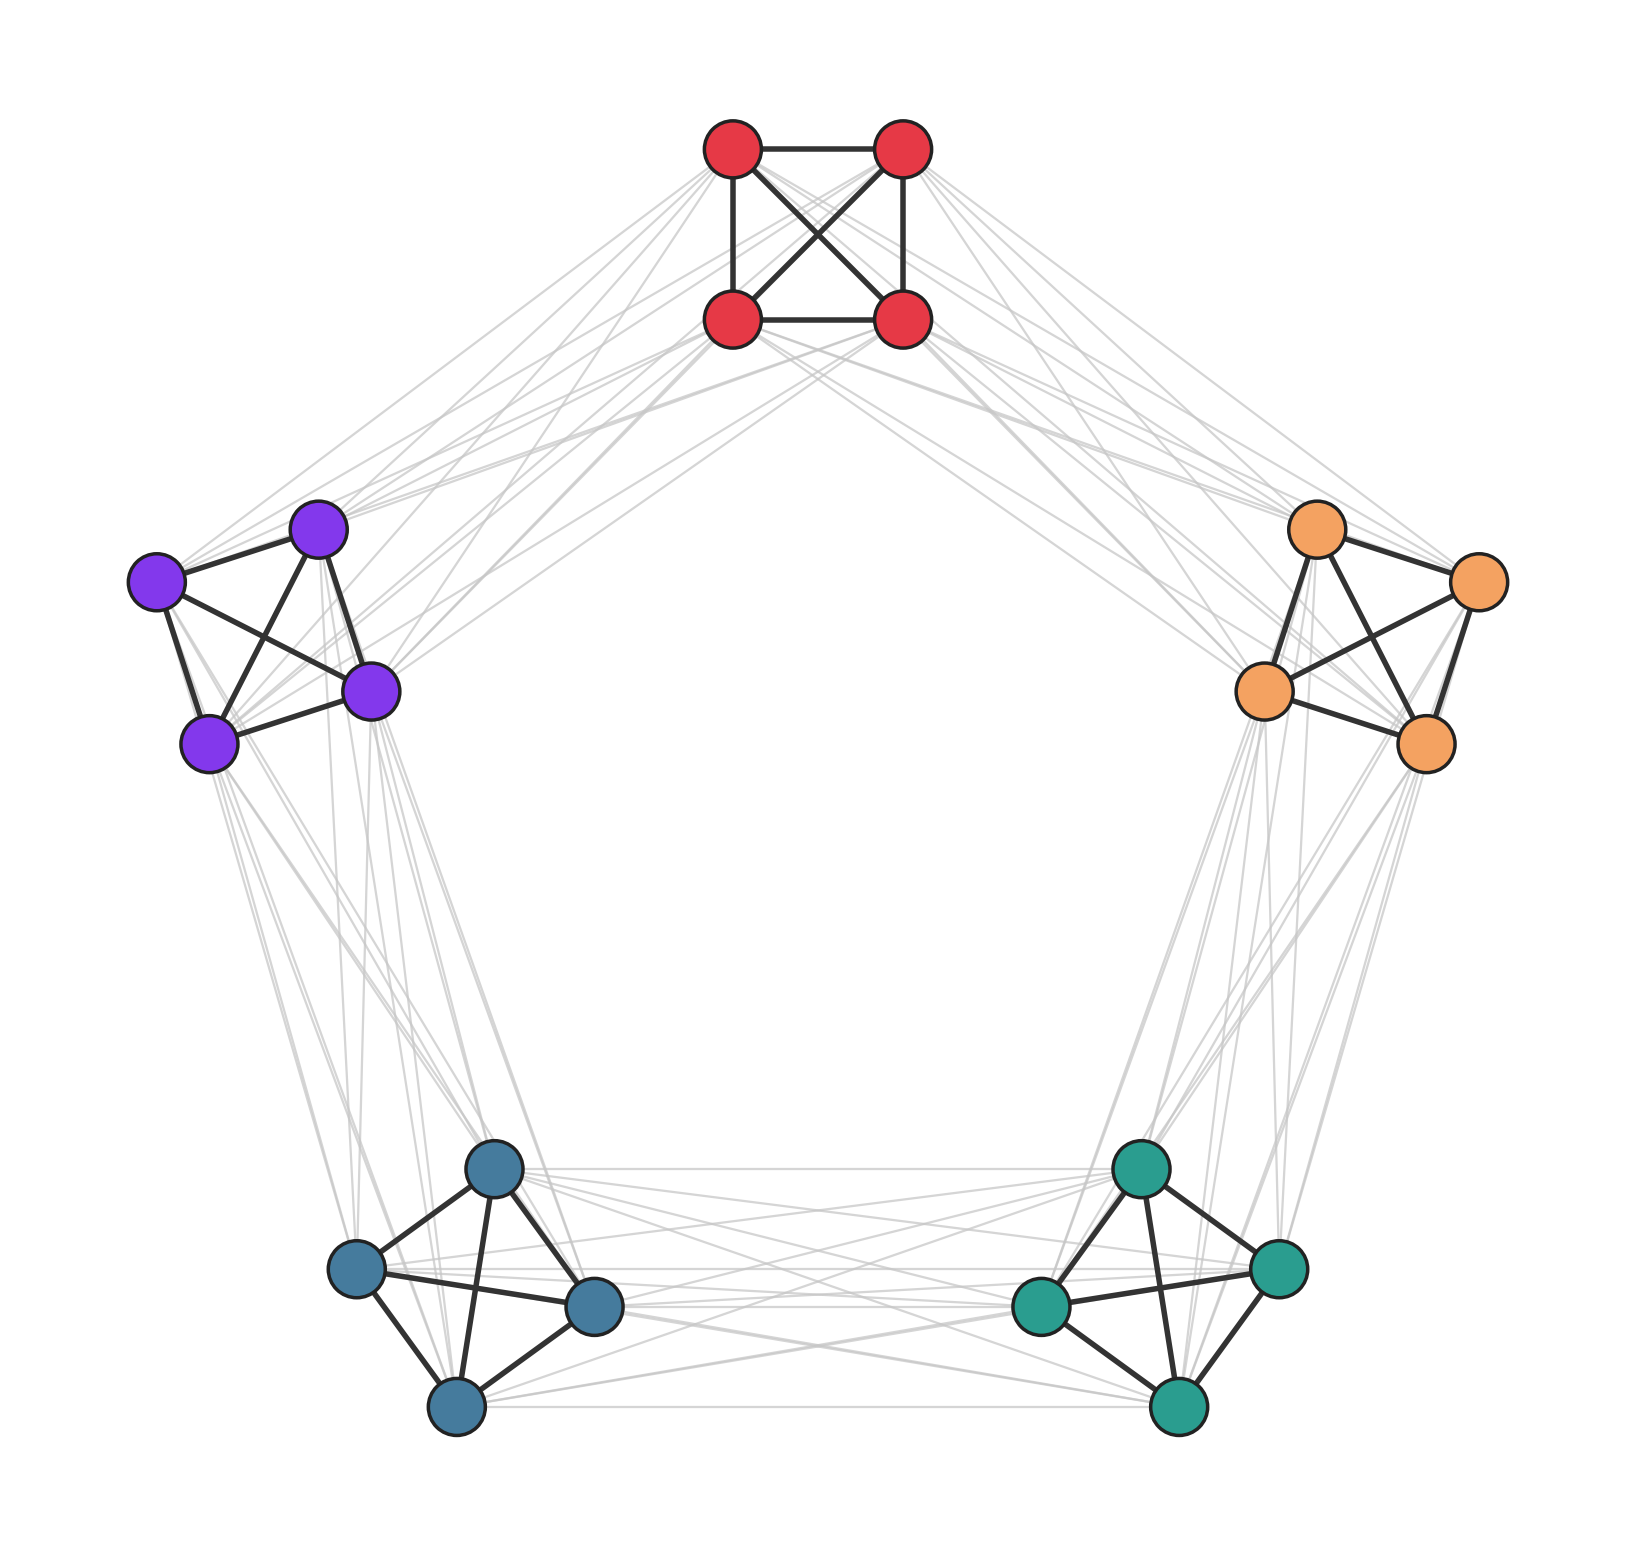
\includegraphics[width=0.42\textwidth]{../../assets/c5k4.png}
\caption{$\blow{C_5}{4}$: five $K_4$ blobs placed on a $5$-cycle, with consecutive blobs
completely joined. It has $20$ vertices, $110$ edges, is $11$-regular, vertex-transitive, and
has diameter $2$.}
\label{fig:carrier}
\end{figure}

The graph of Figure~\ref{fig:carrier} was found on 2026-07-23 while searching WOWII for a
counterexample to Conjecture $85$. It turned out to refute Conjectures $63$ and $85$
simultaneously; Gebendorfer subsequently used the same carrier family to refute $309$
\cite{geb309} and $64$ \cite{geb64}, in both cases crediting the earlier certificate. Four open
conjectures fell to one $20$-vertex graph and its siblings. The point of this paper is not the
count but the explanation: the four kills are four instances of a single arithmetic accident
that the generator's own verification procedure could not have detected.

\section{Preliminaries}\label{sec:prelim}

All graphs are finite, simple and undirected. For a graph $G$ we write $V(G)$, $E(G)$,
$n(G) = |V(G)|$, $\Delta(G)$ and $\delta(G)$ for the maximum and minimum degree, $d_G(u,v)$ for
the distance, $\overline{G}$ for the complement, and $G[S]$ for the subgraph induced by
$S \subseteq V(G)$. We use $\ind(G)$ for the independence number, $\omega(G)$ for the clique
number, $\gamma(G)$, $\gt(G)$, $\gc(G)$ for the domination, total domination and connected
domination numbers, and $\Ls(G)$ for the maximum number of leaves of a spanning tree, so that
$\Ls(G) = n(G) - \gc(G)$ for connected $G$ with $n \ge 3$.

The four ``induced-subgraph numbers'' that carry the argument are, in DeLaVi\~na's notation
\cite{wowiidefs}:
\[
\begin{array}{ll}
\forestnum(G) &= \max\{|S| : G[S] \text{ is a forest}\},\\
\bipnum(G)    &= \max\{|S| : G[S] \text{ is bipartite}\},\\
\treenum(G)   &= \max\{|S| : G[S] \text{ is a tree}\},\\
\pathnum(G)   &= \max\{|S| : G[S] \text{ is a path}\}.
\end{array}
\]
We also use two parity invariants of the WOWII vocabulary. For $v \in V(G)$,
\begin{align*}
\de(v) &= |\{x \in V(G) : d_G(v,x) \text{ is even}\}|,\\
\eh(v) &= |\{xy \in E(G) : d_G(v,x) = d_G(v,y) \text{ and this common value is even}\}|,
\end{align*}
the WOWII invariants \texttt{dist\_even(v)} and \texttt{even horizontal(v)}. The convention
$d_G(v,v) = 0$ makes $v$ itself contribute to $\de(v)$; DeLaVi\~na's page examples imply this
convention, and we verify below (Remark~\ref{rem:conventions}) that our conclusions do not
depend on it. Finally, $n \bmod \Delta$ is an \emph{atomic} invariant of the WOWII vocabulary
(definition~$32$ of \cite{wowiidefs}, defined when $\Delta \ge 2$), not a derived expression;
this matters in Section~\ref{sec:c64}.

\begin{definition}[Clique blow-up]
Let $H$ be a graph with $V(H) = \{1,\dots,k\}$ and let $m \ge 1$. The \emph{clique blow-up}
$H[K_m]$ (the lexicographic product of $H$ with $K_m$) has vertex set
$V(H) \times \{1,\dots,m\}$, with $(i,j)$ adjacent to $(i',j')$ if and only if either $i = i'$
and $j \ne j'$, or $ii' \in E(H)$. We write $B_i = \{i\} \times \{1,\dots,m\}$ for the
\emph{blob} over $i$, and for $S \subseteq V(H[K_m])$ we write $s_i = |S \cap B_i|$ and call
$s = (s_1,\dots,s_k)$ the \emph{profile} of $S$.
\end{definition}

Each $B_i$ induces a $K_m$; if $ii' \in E(H)$ then $B_i \cup B_{i'}$ induces a $K_{2m}$; if
$ii' \notin E(H)$ and $i \ne i'$ then no edge joins $B_i$ to $B_{i'}$.

\section{Pinning}\label{sec:pinning}

Throughout this section $H$ is a graph on $k \ge 1$ vertices, $m \ge 1$, and $G = H[K_m]$.

\begin{lemma}[Blob profile lemma]\label{lem:profile}
Let $S \subseteq V(G)$ be such that $G[S]$ is triangle-free, and let $s$ be its profile. Put
\[
A = \{i \in V(H) : s_i = 2\}, \qquad B = \{i \in V(H) : s_i = 1\}.
\]
Then:
\begin{enumerate}
\item[(i)] $s_i \le 2$ for every $i$;
\item[(ii)] if $i \in A$ then $s_j = 0$ for every $j \in N_H(i)$; in particular $A$ is
independent in $H$ and no edge of $H$ joins $A$ to $B$;
\item[(iii)] $G[S] \cong |A| \cdot K_2 \;\sqcup\; H[B]$ (a disjoint union of $|A|$ copies of
$K_2$ with a copy of the subgraph of $H$ induced by $B$).
\end{enumerate}
Conversely, if $m \ge 2$ and $(A,B)$ is any pair of disjoint subsets of $V(H)$ such that no edge
of $H$ joins a vertex of $A$ to a vertex of $A \cup B$, then some $S \subseteq V(G)$ with
$A = \{i : s_i = 2\}$, $B = \{i : s_i = 1\}$ exists and satisfies
$G[S] \cong |A| \cdot K_2 \sqcup H[B]$.
\end{lemma}

\begin{proof}
(i) $B_i$ induces a clique, so any three vertices of $S \cap B_i$ would induce a triangle.

(ii) Suppose $i \in A$, say $S \cap B_i = \{u,v\}$, and suppose $j \in N_H(i)$ has
$s_j \ge 1$, say $w \in S \cap B_j$. Then $B_i \cup B_j$ induces a clique, so $\{u,v,w\}$
induces a triangle in $G[S]$, a contradiction. If $i,i' \in A$ were adjacent in $H$ we would
have $s_{i'} = 2 \ge 1$, contradicting what we just proved; the same computation excludes edges
from $A$ to $B$.

(iii) By (ii) the vertices of $S$ lying in blobs indexed by $A$ have no neighbours in $S$
outside their own blob, and each such blob contributes exactly two vertices, adjacent to each
other: $|A|$ components isomorphic to $K_2$. Every blob indexed by $B$ contributes exactly one
vertex, and two such vertices, in blobs $i,j$ with $i \ne j$, are adjacent in $G$ if and only if
$ij \in E(H)$. Hence the union of the $B$-blob vertices induces a copy of $H[B]$, and by (ii)
again there are no edges between the two parts.

For the converse, choose for each $i \in A$ two vertices of $B_i$ (possible since $m \ge 2$) and
for each $i \in B$ one vertex of $B_i$. Parts (i)--(iii) of the computation above apply verbatim
and give the stated isomorphism type, which is triangle-free whenever $H[B]$ is.
\end{proof}

\begin{theorem}[Pinning]\label{thm:pinning}
Let $H$ be a graph and $m \ge 1$, $G = H[K_m]$. Then
\begin{enumerate}
\item[(i)] $\ind(G) = \ind(H)$;
\item[(ii)] $\pathnum(G) \le \treenum(G) \le \forestnum(G) \le \bipnum(G) \le 2\ind(H)$;
\item[(iii)] $\bipnum(H) \le \bipnum(G)$ and $\pathnum(H) \le \pathnum(G)$, and the same for
$\forestnum$ and $\treenum$;
\item[(iv)] consequently, if $\pathnum(H) = 2\ind(H)$ then
$\pathnum(G) = \treenum(G) = \forestnum(G) = \bipnum(G) = 2\ind(H)$ for every $m \ge 1$.
\end{enumerate}
In particular each of these four quantities is independent of $m$ under the hypothesis of (iv),
while $n(G) = m \cdot n(H)$ and $\Delta(G) = m(1 + \Delta(H)) - 1$ grow linearly in $m$.
\end{theorem}

\begin{proof}
(i) An independent set of $G$ meets each blob in at most one vertex (blobs are cliques) and its
set of blob indices is independent in $H$ (adjacent blobs are completely joined); hence
$\ind(G) \le \ind(H)$. Conversely one vertex per blob over a maximum independent set of $H$ is
independent in $G$.

(ii) The three left-hand inequalities are immediate from the inclusions
$\{\text{paths}\} \subseteq \{\text{trees}\} \subseteq \{\text{forests}\} \subseteq
\{\text{bipartite graphs}\}$, all four classes being closed under induced subgraphs. For the
last, let $S$ realise $\bipnum(G)$, so $G[S]$ is bipartite with parts $X, Y$. Both $X$ and $Y$
are independent in $G$, so $|X|,|Y| \le \ind(G) = \ind(H)$ by (i), whence
$\bipnum(G) = |X| + |Y| \le 2\ind(H)$.

(iii) If $H[S_0]$ is bipartite (resp.\ a forest, tree, path) for $S_0 \subseteq V(H)$, pick one
vertex from $B_i$ for each $i \in S_0$; the induced subgraph of $G$ on the chosen vertices is
isomorphic to $H[S_0]$.

(iv) By (iii), $\pathnum(G) \ge \pathnum(H) = 2\ind(H)$, and by (ii) all four quantities lie
between $\pathnum(G)$ and $2\ind(H)$.
\end{proof}

\begin{remark}
The inequality $\bipnum(G) \le 2\ind(G)$ used in the proof is elementary and holds for every
graph. The content of Theorem~\ref{thm:pinning} is that composing it with the exact identity
$\ind(H[K_m]) = \ind(H)$ makes the bound \emph{independent of $m$}, and that condition (iv)
identifies when it is met with equality by all four numbers at once.
\end{remark}

\begin{corollary}[Odd cycles]\label{cor:oddcycle}
Let $r \ge 1$, $k = 2r+1$, and $m \ge 1$. Then
\[
\ind(C_k[K_m]) = r
\qquad\text{and}\qquad
\pathnum(C_k[K_m]) = \treenum(C_k[K_m]) = \forestnum(C_k[K_m]) = \bipnum(C_k[K_m]) = 2r .
\]
\end{corollary}

\begin{proof}
$\ind(C_{2r+1}) = r$, and deleting one vertex of $C_{2r+1}$ leaves an induced path on $2r$
vertices, so $\pathnum(C_{2r+1}) = 2r = 2\ind(C_{2r+1})$. Apply Theorem~\ref{thm:pinning}(i)
and (iv).
\end{proof}

For $r = 1$, $k = 5$ this is the pinning statement we need: for every $m \ge 1$,
\begin{equation}\label{eq:pin5}
\ind(\blow{C_5}{m}) = 2,
\qquad
\pathnum = \treenum = \forestnum = \bipnum = 4 \quad\text{on } \blow{C_5}{m}.
\end{equation}
An explicit witness is worth recording, since it is the same set for all four numbers: taking
one vertex from each of $B_0, B_1, B_3, B_4$ gives the induced path
$B_1 - B_0 - B_4 - B_3$ on four vertices (the two chosen vertices in $B_1$ and $B_3$ are
non-adjacent because $1$ and $3$ are at distance $2$ on $C_5$).

Lemma~\ref{lem:profile} gives more than Theorem~\ref{thm:pinning}: it gives the exact value for
an arbitrary hereditary class and shows it stabilises.

\begin{proposition}[Exact values and stabilisation]\label{prop:exact}
Let $\mathcal{F}$ be a class of graphs closed under isomorphism and induced subgraphs, all of
whose members are triangle-free, and let
$\mathcal{F}(G) = \max\{|S| : G[S] \in \mathcal{F}\}$. Then for every $m \ge 2$,
\[
\mathcal{F}(H[K_m]) \;=\; \max\big\{\, 2|A| + |B| \,\big\},
\]
the maximum being over all pairs of disjoint sets $A,B \subseteq V(H)$ such that no edge of $H$
joins $A$ to $A \cup B$ and $|A|K_2 \sqcup H[B] \in \mathcal{F}$;
a quantity that does not depend on $m$. If moreover every member of $\mathcal{F}$ is bipartite,
then $\mathcal{F}(H[K_m]) \le 2\ind(H)$ for every $m \ge 1$.
\end{proposition}

\begin{proof}
Members of $\mathcal{F}$ are triangle-free, so Lemma~\ref{lem:profile} applies to any $S$ with
$G[S] \in \mathcal{F}$, giving $|S| = 2|A| + |B|$ and $G[S] \cong |A|K_2 \sqcup H[B]$ for an
admissible pair $(A,B)$; this proves ``$\le$''. The converse half of Lemma~\ref{lem:profile}
proves ``$\ge$'' when $m \ge 2$. For the last statement, let $(A,B)$ be admissible with
$|A|K_2 \sqcup H[B] \in \mathcal{F}$ bipartite. Then $H[B]$ is bipartite, so it has an
independent set $I$ with $|I| \ge |B|/2$. Since $A$ is independent in $H$ and has no
$H$-neighbour in $B \supseteq I$, the set $A \cup I$ is independent in $H$, whence
$\ind(H) \ge |A| + |B|/2$, i.e.\ $2|A| + |B| \le 2\ind(H)$.
\end{proof}

\begin{example}
For $H = C_5$ the admissible pairs achieving the maximum are $(\emptyset, V \setminus \{i\})$,
giving $P_4$; $(\{i\}, \{i+2,i+3\})$, giving $K_2 \sqcup K_2$; and $(\{i,i+2\}, \emptyset)$,
giving $2K_2$. All three have $2|A| + |B| = 4$. The first is a path, so all four numbers
in~\eqref{eq:pin5} equal $4$; the second and third are forests but not trees, which is why the
value $4$ is realised in three combinatorially different ways.
\end{example}

\subsection{The growing side, and the cliff principle}

Pinning is only half of the mechanism. The other half is that the invariants used as
\emph{correction terms} in the same conjectures are unbounded on the family.

\begin{proposition}[Growth]\label{prop:growth}
Let $H$ be connected, non-complete, with $k = n(H) \ge 3$ vertices, and let $G = H[K_m]$. Then
$n(G) = km$, $G$ is $\big(m(1+\Delta(H)) - 1\big)$-regular when $H$ is regular,
$\omega(G) = m\,\omega(H)$, $\mathrm{diam}(G) = \mathrm{diam}(H)$, and for every
$v = (i,a) \in V(G)$,
\[
\de(v) \;=\; 1 + m\cdot\big|\{\, j \in V(H)\setminus\{i\} : d_H(i,j) \text{ is even} \,\}\big| .
\]
In particular each of $n$, $\Delta$, $\omega$, $\de$ is a linear, unbounded function of $m$
whenever the corresponding coefficient is nonzero.
\end{proposition}

\begin{proof}
The order and regularity are immediate. A clique of $G$ meets only blobs whose indices are
pairwise equal or adjacent in $H$ (non-adjacent blobs have no edges between them) and may
contain a whole blob, so $\omega(G) = m\,\omega(H)$. Distinct vertices of the same blob are
adjacent, and blobs over adjacent vertices of $H$ are completely joined, so
$d_G((i,a),(i',a')) = d_H(i,i')$ whenever $i \ne i'$, and $d_G((i,a),(i,a')) = 1$ for
$a \ne a'$. Since $\mathrm{diam}(H) \ge 2$ this gives $\mathrm{diam}(G) = \mathrm{diam}(H)$ and
the stated formula for $\de$: the vertices at even distance from $(i,a)$ are $(i,a)$ itself
(distance $0$) together with the whole of $B_j$ for each $j \ne i$ with $d_H(i,j)$ even.
\end{proof}

The failure principle is now a one-line consequence, but stating it is the point of the paper.

\begin{proposition}[Cliff principle]\label{prop:cliff}
Let $(G_m)_{m \ge 1}$ be a family of graphs and let $P, \Phi$ be graph invariants such that
$P(G_m) = c$ for all $m$ and $\Phi(G_m) \to \infty$. Then the statement
``$P(G) \ge \Phi(G)$ for all $G$ in the relevant class'' fails on $G_m$ for every $m$ with
$\Phi(G_m) > c$. If $m \mapsto \Phi(G_m)$ is nondecreasing and $m_0$ is the largest index with
$\Phi(G_{m_0}) \le c$, then the statement holds on $G_1, \dots, G_{m_0}$ and fails on every
$G_m$ with $m > m_0$; if in addition $\Phi(G_{m_0}) = c$ then $G_{m_0}$ satisfies the statement
with equality. Symmetrically, if $\Phi(G_m) \to -\infty$ then ``$P(G) \le \Phi(G)$'' fails from
some index onwards, again with equality at the last surviving index when
$\Phi(G_{m_0}) = c$.
\end{proposition}

The observation that matters for conjecture generation is the last clause.
\emph{The last surviving member is an equality case.} A generator whose database stops at
$G_{m_0}$ therefore does not merely fail to refute the candidate; it records the candidate as
\emph{sharp}, and a significance heuristic that rewards sharpness promotes it. The database
boundary and the sharpness signal coincide. We return to this in
Section~\ref{sec:diagnostic}.

\section{The family $\blow{C_5}{m}$}\label{sec:family}

We now specialise to $H = C_5$ and record the exact values of everything used later. Index the
blobs by $\ZZ_5$, so $B_i \cup B_{i+1}$ induces $K_{2m}$ and there are no edges between $B_i$
and $B_{i+2}$.

\begin{proposition}[Basic invariants]\label{prop:basic}
Let $m \ge 1$ and $G = \blow{C_5}{m}$. Then
\[
n(G) = 5m, \quad |E(G)| = \tfrac{5m(3m-1)}{2}, \quad
\mathrm{diam}(G) = \mathrm{rad}(G) = 2,
\]
$G$ is $(3m-1)$-regular and vertex-transitive, and
\[
\ind(G) = 2, \quad \omega(G) = 2m, \quad
\gamma(G) = 2, \quad \gt(G) = 3, \quad \gc(G) = 3, \quad \Ls(G) = 5m - 3 ,
\]
and the local independence number $\lambda(v) := \ind(G[N(v)])$ equals $2$ at every vertex.
\end{proposition}

\begin{proof}
Order, size, regularity and vertex-transitivity are immediate from the construction
($\deg = (m-1) + 2m$; the automorphism group contains the dihedral action on blobs and all
within-blob permutations, acting transitively). Non-adjacent vertices lie in blobs at $C_5$-distance
$2$ and have a common neighbour in an intermediate blob, so $\mathrm{diam}(G) = 2$; every vertex
has non-neighbours, so $\mathrm{rad}(G) = 2$. $\ind(G) = \ind(C_5) = 2$ and $\omega(G) = 2m$ by
Theorem~\ref{thm:pinning}(i) and Proposition~\ref{prop:growth}.

For domination: a single vertex of $B_i$ dominates exactly $B_{i-1} \cup B_i \cup B_{i+1}$, so
$\gamma(G) \ge 2$, and $\{u,w\}$ with $u \in B_i$, $w \in B_{i+2}$ dominates all five blobs, so
$\gamma(G) = 2$. Since a total dominating set of size $2$ must be an edge $uv$ with
$N(u) \cup N(v) = V(G)$, and the union of two closed blob-neighbourhoods
$\{i-1,i,i+1\} \cup \{i',i'-1,i'+1\}$ with $i' \in \{i, i \pm 1\}$ never covers $\ZZ_5$, we get
$\gt(G) \ge 3$; and $\{u,v,w\}$ with $u \in B_0$, $v \in B_1$, $w \in B_2$ is total dominating
(their blob neighbourhoods cover $\ZZ_5$ and each of the three has one of the others as a
neighbour), so $\gt(G) = 3$. A connected dominating set of size $2$ is in particular a
dominating set inducing an edge, so its blobs are equal or adjacent and again fail to cover
$\ZZ_5$; the set $\{u,v,w\}$ above is connected and dominating, so $\gc(G) = 3$ and
$\Ls(G) = n - \gc = 5m - 3$.

Finally, for $v \in B_i$ we have $N(v) = (B_i \setminus \{v\}) \cup B_{i-1} \cup B_{i+1}$. An
independent set of $G[N(v)]$ contains at most one vertex of each blob and its set of blob
indices is independent in the path $(i-1,\,i,\,i+1)$ induced by $C_5$ on those three indices;
hence $\lambda(v) \le 2$. Taking one vertex of $B_{i-1}$ and one of $B_{i+1}$, which are
non-adjacent because $i-1$ and $i+1$ are at $C_5$-distance $2$, gives $\lambda(v) = 2$, for
every $m \ge 1$.
\end{proof}

\begin{proposition}[Parity, residue and complement]\label{prop:parity}
Let $m \ge 1$, $G = \blow{C_5}{m}$, and $v \in V(G)$. Then
\[
\de(v) = 2m+1, \qquad
\eh(v) = m(2m-1), \qquad
\overline{G} \;\cong\; C_5[\overline{K_m}] ,
\]
$\overline{G}$ is $2m$-regular, triangle-free, of diameter $2$, and
$\min_{e \in E(\overline{G})} |N_{\overline{G}}(e)| = 4m$, where
$N_{\overline{G}}(xy) = N_{\overline{G}}(x) \cup N_{\overline{G}}(y)$. Moreover
\[
n \bmod \Delta \;=\; 5m \bmod (3m-1) \;=\; 2m+1 \qquad \text{for every } m \ge 3,
\]
while $5 \bmod 2 = 1$ for $m = 1$ and $10 \bmod 5 = 0$ for $m = 2$.
\end{proposition}

\begin{proof}
Let $v \in B_i$. Vertices at distance $0$ or $2$ from $v$ are $v$ itself and all of
$B_{i+2} \cup B_{i-2}$, giving $\de(v) = 1 + 2m$; the remaining $3m-1$ vertices are at distance
$1$. The vertex pairs at equal even distance from $v$ are the pairs inside
$B_{i+2} \cup B_{i-2}$ (both at distance $2$); since $i+2$ and $i-2 = i+3$ are adjacent on
$C_5$, this set induces $K_{2m}$, contributing $\binom{2m}{2} = m(2m-1)$ edges, and $v$ has no
neighbour at distance $2$ from itself, so $\eh(v) = m(2m-1)$. (The same value is obtained under
the weaker reading ``both endpoints at even distance'', because $v$ is isolated from
$B_{i+2} \cup B_{i-2}$.)

In $\overline{G}$, $(i,j)$ and $(i',j')$ are adjacent exactly when $i - i' \equiv \pm 2
\pmod 5$; since $\{\pm 2\}$ generates a $5$-cycle on $\ZZ_5$, $\overline{G}$ is the blow-up of a
$5$-cycle by independent sets, so it is $2m$-regular, triangle-free (an odd cycle blow-up by
independent sets contains a triangle only if the base does) and of diameter $2$. Let
$xy \in E(\overline{G})$ with $x \in B_i$, $y \in B_{i+2}$. Then
$N_{\overline{G}}(x) = B_{i+2} \cup B_{i-2}$ and
$N_{\overline{G}}(y) = B_{i+4} \cup B_{i}$; these four blobs are distinct, so
$|N_{\overline{G}}(x) \cup N_{\overline{G}}(y)| = 4m$, independently of the edge chosen.

Finally $5m = 1 \cdot (3m-1) + (2m+1)$ and $0 \le 2m+1 < 3m-1$ exactly when $m > 2$.
\end{proof}

\begin{remark}\label{rem:conventions}
Two conventions in the WOWII vocabulary are ambiguous in the published text: whether $v$ counts
in $\de(v)$, and whether the endpoints of $e$ count in $N(e)$. Under the alternative
conventions, $\de(v) = 2m$ and $|N_{\overline{G}}(e)| = 4m - 2$. All four refutations in
Section~\ref{sec:cliff} survive all combinations of these conventions; the per-conjecture
verdicts for every combination are recorded in the sweep data
(Section~\ref{sec:repro}).
\end{remark}

Combining Proposition~\ref{prop:basic}, Proposition~\ref{prop:parity} and~\eqref{eq:pin5}, the
family exhibits the mechanism in its purest form:
\begin{center}
\begin{tabular}{ll}
\toprule
\textbf{pinned (constant in $m$)} & \textbf{growing (linear or quadratic in $m$)}\\
\midrule
$\ind = 2$ & $n = 5m$, \quad $\Delta = \delta = 3m-1$, \quad $\omega = 2m$\\
$\pathnum = \treenum = \forestnum = \bipnum = 4$ & $\de = 2m+1$, \quad $n \bmod \Delta = 2m+1$ $(m \ge 3)$\\
$\gamma = 2$, \; $\gt = 3$, \; $\gc = 3$ & $\eh = m(2m-1)$, \quad $\min|N_{\overline G}(e)| = 4m$\\
$\mathrm{diam} = \mathrm{rad} = 2$, \; $\lambda(v) = 2$ & $\Ls = 5m-3$, \quad $\deg_{\mathrm{avg}}(\overline{G}) = 2m$\\
\bottomrule
\end{tabular}
\end{center}

\section{Four conjectures, four cliffs}\label{sec:cliff}

We now state the four WOWII conjectures verbatim as transcribed from DeLaVi\~na's page
\cite{wowii} and evaluate them on the family. The transcriptions, including the unbalanced
brackets in $64$, reproduce the page as published; the transcription audit and the recovery of
DeLaVi\~na's own invariant-definition database are described in Section~\ref{sec:corpus}.

\subsection{Conjecture 63}

\begin{quote}
\textbf{WOWII 63} (page marker \texttt{O}, dated Mar.\ 25, 2004). \emph{If $G$ is a simple
connected graph, then}
$\forestnum(G) \ge \big\lceil (\min_v \de(v) + \bipnum(G) + 1)/3 \big\rceil$.
\end{quote}

\begin{theorem}\label{thm:63}
On $G = \blow{C_5}{m}$ the right-hand side of WOWII 63 equals
$\lceil (2m+6)/3 \rceil$. Hence Conjecture 63 holds on $\blow{C_5}{m}$ for $m \le 3$, with
equality for $m \in \{2,3\}$, and fails for every $m \ge 4$.
\end{theorem}

\begin{proof}
By Proposition~\ref{prop:parity} $\min_v \de(v) = 2m+1$, and by~\eqref{eq:pin5}
$\bipnum = 4$ and $\forestnum = 4$. So the right-hand side is
$\lceil (2m+1+4+1)/3\rceil = \lceil (2m+6)/3 \rceil$, which is $\le 4$ exactly when
$2m + 6 \le 12$, i.e.\ $m \le 3$, and equals $4$ exactly when $10 \le 2m+6 \le 12$, i.e.\
$m \in \{2,3\}$.
\end{proof}

\subsection{Conjecture 85}

\begin{quote}
\textbf{WOWII 85} (page marker \texttt{O}, dated Apr.\ 04, 2004). \emph{If $G$ is a simple
connected graph, then} $\treenum(G) \ge \big\lceil \sqrt{1 + 2\min_v \de(v)} \big\rceil$.
\end{quote}

\begin{theorem}\label{thm:85}
On $G = \blow{C_5}{m}$ the right-hand side of WOWII 85 equals $\lceil \sqrt{4m+3} \rceil$.
Hence Conjecture 85 holds on $\blow{C_5}{m}$ for $m \le 3$, with equality for
$m \in \{2,3\}$, and fails for every $m \ge 4$.
\end{theorem}

\begin{proof}
$1 + 2(2m+1) = 4m+3$, and $\treenum = 4$. Now $\lceil\sqrt{4m+3}\rceil \le 4$ iff
$4m + 3 \le 16$ iff $m \le 3$ (as $m$ is an integer), and $\lceil\sqrt{4m+3}\rceil = 4$ iff
$9 < 4m+3 \le 16$ iff $m \in \{2,3\}$.
\end{proof}

\subsection{Conjecture 64}\label{sec:c64}

\begin{quote}
\textbf{WOWII 64} (page marker \texttt{O}, dated Mar.\ 25, 2004). \emph{If $G$ is a simple
connected graph, then} $\forestnum(G) \ge \mathrm{CEIL}[(\sqrt{\,\ind(G) \cdot (1 + (n \bmod
\Delta(G))\,}\,]$.
\end{quote}

The bracketing on the page is unbalanced. The reading we use is
\[
\forestnum(G) \;\ge\; \Big\lceil \sqrt{\ind(G)\,\big(1 + (n \bmod \Delta(G))\big)} \Big\rceil ,
\]
which is pinned by the page's own \texttt{printDefinitions} link with arguments
$(41,5,32,16,0)$: the constituents are declared to be the forest number, $\ind$, the
\emph{atomic} invariant ``$n$ modulus maximum degree'' (definition $32$), and the ceiling
function.

\begin{theorem}\label{thm:64}
On $G = \blow{C_5}{m}$ with $m \ge 3$, the right-hand side of WOWII 64 equals
$\lceil 2\sqrt{m+1} \rceil$; for $m \in \{1,2\}$ it equals $2$. Hence Conjecture 64 holds on
$\blow{C_5}{m}$ for $m \le 3$, with equality at $m = 3$, and fails for every $m \ge 4$.
\end{theorem}

\begin{proof}
For $m \ge 3$, Proposition~\ref{prop:parity} gives $n \bmod \Delta = 2m+1$, and
$\ind = 2$, so the radicand is $2(2m+2) = 4(m+1)$ and the right-hand side is
$\lceil 2\sqrt{m+1}\rceil$. This is $\le 4$ iff $4(m+1) \le 16$ iff $m \le 3$, with equality
exactly at $m = 3$ (where $4(m+1) = 16$ is a perfect square). For $m = 1$ the radicand is
$2(1+1) = 4$ and for $m = 2$ it is $2(1+0) = 2$, giving right-hand sides $2$ and $2$. Since
$\forestnum = 4$ throughout, the claim follows.
\end{proof}

\subsection{Conjecture 309}

\begin{quote}
\textbf{WOWII 309} (page marker \texttt{O}, dated Mar.\ 1, 2007). \emph{If $G$ is a simple
connected graph such that $n(G) > 2$, then}
\[
\gt(G) \;\le\; \tfrac12\Big[\max_{v \in V(G)}\big\{\de(v) - \eh(v)\big\}
\;+\; \min_{e \in E(\overline{G})} |N_{\overline{G}}(e)|\Big].
\]
\end{quote}

\begin{theorem}\label{thm:309}
On $G = \blow{C_5}{m}$ the right-hand side of WOWII 309 equals
$\tfrac12(-2m^2 + 7m + 1)$. Hence Conjecture 309 holds on $\blow{C_5}{m}$ for
$m \in \{1,2\}$, with equality at $m = 1$, and fails for every $m \ge 3$, with margin
$\tfrac12(2m-5)(m-1) \to \infty$.
\end{theorem}

\begin{proof}
By Proposition~\ref{prop:parity} and vertex-transitivity, $\de(v) - \eh(v) = 2m+1 - m(2m-1) =
-2m^2 + 3m + 1$ for every $v$, and $\min_e |N_{\overline{G}}(e)| = 4m$. So the right-hand side
is $\tfrac12(-2m^2+3m+1+4m) = \tfrac12(-2m^2+7m+1)$. With $\gt = 3$
(Proposition~\ref{prop:basic}), the conjecture asserts $6 \le -2m^2+7m+1$, i.e.\
$2m^2 - 7m + 5 \le 0$, i.e.\ $(2m-5)(m-1) \le 0$, which for positive integers $m$ holds exactly
for $m \in \{1,2\}$, with equality only at $m = 1$.
\end{proof}

Theorem~\ref{thm:309} recovers Gebendorfer's closed forms \cite{geb309} by an independent
derivation; the smallest member of the family that refutes $309$ is $\blow{C_5}{3}$, of order
$15$, where the conjecture asserts $3 \le 2$.

\section{The cliff table and the $m = 3$ diagnostic}\label{sec:diagnostic}

Table~\ref{tab:cliff} collects the four theorems of Section~\ref{sec:cliff}.

\begin{table}[t]
\centering\small
\begin{tabular}{rrrcrrrrl}
\toprule
$m$ & $n$ & $\Delta$ & pinned & $\min\de$ &
RHS$_{63}$ & RHS$_{85}$ & RHS$_{64}$ & RHS$_{309}$ \\
\midrule
$1$ & $5$  & $2$  & $4$ & $3$  & $3$ & $3$ & $2$ & $3$\\
$2$ & $10$ & $5$  & $4$ & $5$  & $\mathbf{4}$ & $\mathbf{4}$ & $2$ & $7/2$\\
$3$ & $15$ & $8$  & $4$ & $7$  & $\mathbf{4}$ & $\mathbf{4}$ & $\mathbf{4}$ & $2$\\
$4$ & $20$ & $11$ & $4$ & $9$  & $5$ & $5$ & $5$ & $-3/2$\\
$5$ & $25$ & $14$ & $4$ & $11$ & $6$ & $5$ & $5$ & $-7$\\
\bottomrule
\end{tabular}
\caption{The discretization cliff on $\blow{C_5}{m}$. The column ``pinned'' is the common value
$\forestnum = \bipnum = \treenum = \pathnum = 4$; the left-hand side of $63$ and $64$ is
$\forestnum$, of $85$ is $\treenum$, and of $309$ is $\gt = 3$. A conjecture holds at $m$ iff
its RHS is at most its LHS. Bold entries are exact equalities. At $m=1,2$ all four hold, with
$309$ tight at $m=1$ and $63,85$ tight at $m=2$; at $m=3$ conjectures $63$, $85$, $64$ are
simultaneously tight while $309$ already fails; for every $m \ge 4$ all four fail. Columns
$63$, $85$, $64$ are printed by \texttt{scripts/family\_sweep.py}; column $309$ is
Theorem~\ref{thm:309}. All entries are re-derived by
\texttt{verify\_paper\_claims.py} (Section~\ref{sec:repro}).}
\label{tab:cliff}
\end{table}

Three features of the table are worth isolating.

\paragraph{(a) Simultaneity.} Three conjectures from two different sections of the list
($63$ and $64$ sit in ``2nd run on lower bounds on the forest number''; $85$ in ``lower bounds
on the tree number'') have their last surviving member at the \emph{same} index $m = 3$, and all
three are attained there with equality. They are not the same statement, and they are not
rescaled versions of one another: their right-hand sides grow like $\tfrac23 m$, $2\sqrt{m}$ and
$2\sqrt{m}$ respectively, and are built from different invariants --- $\de$ alone; $\de$ under a
square root; and $\ind$ together with the residue $n \bmod \Delta$. The synchronisation comes
from the pinning: all three lower-bound a quantity stuck at $4$, so three unbounded functions
that are still at most $4$ when $m = 3$ have all passed it by $m = 4$. Simultaneity is therefore
what the mechanism predicts, and it is the reason a single family can clear several entries of a
corpus at once rather than one.

\paragraph{(b) The equalities are partly manufactured by the rounding.} At $m=3$ the three
right-hand sides are $(2\cdot 3+6)/3 = 4$ exactly (the numerator is divisible by $3$),
$\lceil\sqrt{15}\rceil = 4$ because $15$ falls in the gap $(9,16]$, and $\sqrt{2\cdot 8} = 4$
exactly because $16$ is a perfect square. Two of these equalities are genuine, in the sense that
they survive deleting the ceiling; the third ($85$ at $m=3$) exists only because of it, as do
both equalities at $m = 2$. Of the five bold entries in Table~\ref{tab:cliff} for $63$, $85$ and
$64$, three are artefacts of rounding and two are not.

Deleting the ceilings does \emph{not} move the failure thresholds: $4 \ge (2m+6)/3$,
$4 \ge \sqrt{4m+3}$ and $4 \ge 2\sqrt{m+1}$ each hold exactly for integers $m \le 3$. So the
rounding does not create the cliff --- the pinning and the growth do that --- but it creates
three of the five equalities \emph{at the edge of the cliff}, and the equality is precisely what
a Dalmatian-style significance heuristic reads. This is the sense in which the phenomenon is a
\emph{discretization} cliff: the discretization converts a bound with small slack, on the last
few members before the failure, into a bound that looks sharp.

\paragraph{(c) The last surviving member is an extremal witness.} This is
Proposition~\ref{prop:cliff}'s last clause instantiated. A database containing
$\blow{C_5}{1}$, $\blow{C_5}{2}$ and $\blow{C_5}{3}$ but not $\blow{C_5}{4}$ would report all
three of $63$, $85$, $64$ as true and sharp. That is the strongest possible endorsement a
Graffiti-type filter can give.

\medskip

We therefore propose the following diagnostic, and we state it as a heuristic rather than a
theorem.

\begin{quote}
\textbf{Diagnostic.} Let $\mathcal{G}$ be a family of graphs indexed so that some invariant is
pinned along it. If a machine-generated bound is attained with equality on the largest member of
$\mathcal{G}$ present in the generator's database, and if its right-hand side is a nonconstant
function of the index, then the bound is a candidate for refutation by the next member.
\end{quote}

The diagnostic has real content only if the two hypotheses can be checked without knowing the
database. The first can: one computes the slack of the bound on successive members of a
candidate family and looks for a zero. The second can: one checks whether the invariants
occurring on the right-hand side are among those that grow. Both are cheap. What we do
\emph{not} claim is that following the diagnostic locates new counterexamples at a useful rate;
see Section~\ref{sec:limits}.

\begin{remark}[On the database boundary]
It is tempting to say that Graffiti.pc's verification database stopped at some order $n_0$ with
$15 \le n_0 < 20$. We have no evidence for any particular $n_0$: the exact contents of the
database used for the 2004--2007 WOWII runs are not published, as far as we can determine
\textbf{[CITATION NEEDED]}. What is verifiable is a lower bound on where the failure begins:
each of $63$, $85$ and $64$ holds on all $995$ connected graphs of order at most $7$ and on a
list of standard larger graphs, and $309$ holds on all $989$ applicable connected graphs of
order $3$ to $7$ with $36$ exact equalities among them (Section~\ref{sec:repro}). Neither do we
claim that $\blow{C_5}{3}$ itself was in the database; the equality at $m=3$ is a fact about the
family, and its coincidence with a plausible database horizon is a hypothesis about why the
conjectures were emitted.
\end{remark}

\section{The family against the whole WOWII corpus}\label{sec:corpus}

\subsection{Protocol}

The WOWII page was transcribed into $522$ machine-readable records ($521$ distinct identifiers;
one entry, $434$a, occurs twice on the page). Each record carries the verbatim statement, the
page's status marker, and its section. The corpus splits as $220$ open, $139$ already refuted by
others, and $163$ proved or otherwise resolved.

Evaluating a WOWII statement on a concrete graph is not mechanical, for two reasons. First, the
page was authored in a Symbol-font HTML dialect and several statements are ambiguous in
precedence or in the scope of a set-valued argument. Second, some statements are simply corrupt
as published. We handled both as follows.

\begin{enumerate}
\item \textbf{Reading enumeration.} For each ambiguous statement we enumerated all plausible
readings and evaluated every one; verdicts are reported per reading.
\item \textbf{Database-sanity gate.} A reading is discarded if it is violated by a graph that
was certainly available to the generator --- concretely, by one of the $995$ connected graphs of
order $2 \le n \le 7$, or by a standard small named graph. A conjecture the program emitted
cannot be false on the program's own trivial range; a reading that is false there is a
mis-transcription, not a discovery. This gate discarded readings for $10$ statements and
disqualified $3$ statements entirely (below).
\item \textbf{Invariant definitions.} All invariants were implemented against DeLaVi\~na's own
definition database \texttt{wowIIdefs.js}, recovered from an archived snapshot of the site, so
that ``$\de$'', ``$\eh$'', ``$N(e)$'', ``$\Ls$'', ``maxine'' and the rest carry the author's
definitions rather than ours.
\item \textbf{Adversarial re-verification.} Every \texttt{VIOLATED} verdict was recomputed by a
second, independently written code path whose stated objective was to \emph{save} the
conjecture. Two of the six initial open-list violations did not survive this step
(see~\ref{sec:corrupt}).
\end{enumerate}

\subsection{Results}

Against $\blow{C_5}{4}$ the outcome is:

\begin{center}\small
\begin{tabular}{lrrrrl}
\toprule
subcorpus & records & holds & n/a & violated & \\
\midrule
open    & $220$ & $167$      & $47$ & $6$       & $4$ claimed, $2$ rejected (\S\ref{sec:corrupt})\\
refuted & $139$ & $101$      & $29$ & $8\,(+1)$ & retro-kills; $(+1)$ reading-dependent (\#77)\\
proved  & $163$ & $98{+}19$  & $45$ & $1$       & $19$ at zero slack; the $1$ is a defect\\
\midrule
total   & $522$ &            &      &           & \\
\bottomrule
\end{tabular}
\end{center}

\paragraph{The four open kills.} $63$, $85$, $64$, $309$; Section~\ref{sec:cliff}. Conjectures
$63$ and $85$ were first refuted by $\blow{C_5}{4}$ in July 2026; $64$ and $309$ were
subsequently refuted by Gebendorfer using the same carrier family, with the earlier certificate
credited in both notes \cite{geb64,geb309}. Formal Lean~4 certificates without \texttt{sorry}
exist for all four.

\paragraph{Eight retro-kills.} Among the $139$ conjectures already refuted by others,
$\blow{C_5}{4}$ is a counterexample to $24$, $25$, $46$, $49$, $52$, $54$, $55$, $56$ (and,
under one of two readings, $77$). These are not novelty claims --- the conjectures were dead
already. They are evidence about the mechanism, because they are exactly the predicted shape.
Table~\ref{tab:retro} lists them with the pinned left-hand side and the growing right-hand
term.

\begin{table}[t]
\centering
\small
\begin{tabular}{rlllrr}
\toprule
\# & statement (as transcribed) & pinned LHS & growing term & LHS & RHS \\
\midrule
$24$ & $\bipnum \ge \lambda + \lceil \min\de/3\rceil$ & $\bipnum = 4$ & $\de = 2m+1$ & $4$ & $5$\\
$25$ & $\bipnum \ge 2\lceil (1+\min\de)/3\rceil$ & $\bipnum = 4$ & $\de = 2m+1$ & $4$ & $8$\\
$46$ & $\forestnum \ge \lfloor \pathnum - 1 + \tfrac13(n \bmod \Delta)\rfloor$ & $\forestnum = 4$ & $n \bmod \Delta = 2m+1$ & $4$ & $6$\\
$49$ & $\forestnum \ge \lceil 2 + \tfrac16 \mathrm{length}(\overline{G})\rceil$ & $\forestnum = 4$ & $\mathrm{length}(\overline{G}) = 2m\sqrt{5m}$ & $4$ & $8$\\
$52$ & $\forestnum \ge \lceil \tfrac12(dd + 1 + (n \bmod \Delta))\rceil$ & $\forestnum = 4$ & $n \bmod \Delta = 2m+1$ & $4$ & $6$\\
$54$ & $\forestnum \ge \lceil \mathrm{dist_{avg}}(V) + \tfrac12\min\de \rceil$ & $\forestnum = 4$ & $\de = 2m+1$ & $4$ & $6$\\
$55$ & $\forestnum \ge \lceil \min\de - 1 + |N(A)|/3\rceil$ & $\forestnum = 4$ & $\de,\;|N(A)| = 5m$ & $4$ & $15$\\
$56$ & $\forestnum \ge \lceil \sqrt{\mathrm{dist_{max}}(A)\,(1+\deg_{\mathrm{avg}}(\overline{G}))}\rceil$ & $\forestnum = 4$ & $\deg_{\mathrm{avg}}(\overline{G}) = 2m$ & $4$ & $5$\\
\bottomrule
\end{tabular}
\caption{The eight retro-kills on $\blow{C_5}{4}$. In every case a pinned induced-subgraph number
is lower-bounded by a term that Proposition~\ref{prop:growth} makes unbounded in $m$. Here
$\lambda = \max_v \ind(G[N(v)]) = 2$, $dd$ is the number of distinct degrees ($=1$, the graph is
regular), $A$ is the set of minimum-degree vertices ($= V$), and
$\mathrm{length}(G) = \sqrt{\sum_v \deg(v)^2}$. LHS/RHS columns are the values at $m = 4$ from
\texttt{results/refuted\_sweep/}.}
\label{tab:retro}
\end{table}

\paragraph{The sharpness gallery.} This is the larger half of the data and, we argue, the more
informative half. Against the corpus, $\blow{C_5}{4}$ attains zero slack in:
\begin{itemize}
\item \textbf{$19$ proved theorems} of the corpus: $4$, $7$, $15$, $16$, $18$, $37$, $57$, $68$,
$89$, $94$, $99$, $173$, $382$a, $409$a, $411$, $420$a, $451$, $452$, $458$. For instance
$\bipnum = 4 = 2\,\mathrm{rad}(G) = 2\ind(G)$ and $\ind(G) = 2 = \bipnum(G) - \min_v \lambda(v)$
hold simultaneously, so several of these theorems are extremal on the same graph at once.
\item \textbf{$12$ conjectures open at the time of the sweep}, under gate-surviving readings:
$19$, $174$, $176$, $181$, $182$, $183$, $184$, $185$, $382$e, $422$b, $430$a, $438$b. (Three of
these have since moved: $174$ was refuted by a third party in July 2026 by an $11$-vertex graph;
$438$b was subsequently proved; $176$, $181$ and $430$a were later refuted, by other graphs, in
work not reported here.)
\item \textbf{Four already-refuted bounds}: $219$, $289$, $424$, $430$b.
\item One of the three conjectures ($137$) that the July 2026 community transcription of the
page omitted altogether and that our audit recovered: $\pathnum = 4 = 4/p(\overline{G})$, the
complement being Hamiltonian.
\end{itemize}

That is roughly three dozen zero-slack coincidences for one graph. Some of them have a
common explanation and it is instructive. WOWII $173$ is a theorem of DeLaVi\~na and Waller
\cite{delavinawaller2008}: $\Ls(G) + \bipnum(G) \ge n(G) + 1$ for every nontrivial connected
$G$. If $\mathrm{diam}(G) = 2$ then $G^2 = K_n$, and under the gate-surviving readings the
right-hand sides of $176$, $182$, $183$, $184$ and $185$ all collapse to exactly $n+1$. Our
family has $\Ls + \bipnum = (5m-3) + 4 = 5m + 1 = n + 1$: it lies on the sharpness locus of a
known theorem, and the five later conjectures are machine-generated attempted strengthenings
whose correction terms vanish there. No diameter-two graph can refute any of them. This is a
concrete instance of a general and, we think, under-appreciated point: a large block of
zero-slack results on one carrier can be a signal that several published conjectures share a
single already-proved baseline, which is diagnostic information about the corpus rather than
about the graph.

\subsection{Corpus defects, stated rather than exploited}\label{sec:corrupt}

Four entries of the corpus are corrupt as published, and we do not count them.

\begin{itemize}
\item \textbf{$412$f} and \textbf{$448$b} are violated by $\blow{C_5}{4}$ under the literal
published wording --- and also by $K_3$ and by $C_4$ respectively, i.e.\ by graphs certainly
inside the generator's verification range. Under every repair of the wording that is clean on
the $995$-graph gate, $\blow{C_5}{4}$ satisfies them. As published, $412$f is violated by $62\%$
of all connected graphs of order at most $7$. A ``refutation'' of a page typo is empty, so these
are recorded as \texttt{NOT A USABLE KILL}. We checked archived captures back to 2010 (for
$412$f) and 2016 (for $448$b) and found the same corrupt wording already present, so the
corruption is not recent.
\item \textbf{$401$b}, on which $\blow{C_5}{4}$ is exactly tight, has a transcription that is
violated by $K_{1,5}$ and $K_{1,6}$; its tightness is therefore not interpretable and it is
excluded from the sharpness count above.
\item \textbf{Theorem $97$} of the corpus, as transcribed, reads
$\ind(G) \le \max_v \lambda(v) - \delta(\overline{G})$ and is falsified by $\blow{C_5}{4}$ ---
and by $C_5$ and by the Petersen graph. The published minus sign is almost certainly a plus lost
in the Symbol-font encoding; with a plus the statement is true and holds here with slack $8$.
This is the single \texttt{ANOMALY\_VIOLATED} entry in the proved subcorpus and it is a
transcription artefact, not a counterexample to a theorem.
\end{itemize}

We also record, as a caveat on any exhaustive claim about this corpus, that the July 2026
community parse of the page missed three open conjectures entirely ($136$, $137$, $138$; their
identifier cells are split across HTML tags in a way that defeats a naive parser) and that the
page itself was edited on 2026-08-06, moving ten conjectures from open to resolved. Any
statement of the form ``all $N$ open WOWII conjectures'' is a statement about a snapshot.

\subsection{Where the carrier is useless}

The other side of an exhaustive sweep is knowing the boundary of a tool's reach. On
$\blow{C_5}{4}$: the $47$ ``not applicable'' open records are almost all conjectures with tree,
bipartite, triangle-free, planar or sparse hypotheses, which the graph fails; the
well-total-dominated characterisations $314$--$328$ all escape vacuously (the graph is not
well-total-dominated, but every antecedent fails on it, with $314$ saved only by the graph's
$260$ triangles); and the remaining $\gt$ upper bounds $305$, $308$, $310$ hold with slack $5$
or more. The carrier is a specialised instrument: it is productive precisely against
machine-generated inequalities that combine a pinned induced-subgraph or domination invariant
with a density/parity correction, and it is inert everywhere else. A separate sweep of $71$
AutoGraphiX targets produced no gate-surviving violation ($45$ hold, $24$ have unrecoverable
definitions, one is inapplicable and already proved, and the single apparent violation fails the
database-sanity gate), and a sweep of a set of human structural conjectures produced none
either.

\section{Limitations, and what this is not}\label{sec:limits}

\paragraph{This is not a counterexample engine.} We have exhibited one family, analysed one
base graph $H = C_5$ in detail, and refuted four open conjectures in one corpus. The pinning
theorem is general and cheap to instantiate for other $H$ (odd cycles all work, by
Corollary~\ref{cor:oddcycle}), but the \emph{other} half of the mechanism --- the requirement
that the target corpus contains bounds combining a pinned invariant with a growing one --- is a
property of the corpus, not of the construction. We have no evidence that this regime is common
outside machine-generated inequality corpora. Applied to human structural conjectures the same
carrier produced nothing.

\paragraph{We do not claim prospective navigation.} A natural conjecture suggested by
Section~\ref{sec:diagnostic} is that the equality data can be used \emph{forward}: identify the
invariant that keeps a family pinned to an equality wall, construct a family that changes that
invariant while preserving the rest of the extremal structure, and cross. We have one
suggestive instance and we present it as exactly that, with no efficacy claim attached.

\begin{observation}[Suggestive follow-up; not a result of this paper]
The whole blow-up family saturates the ``$\Ls + \bipnum$'' cluster of WOWII (conjectures
$174$--$186$) at exact equality without ever crossing it, and every member has
$\ind = \lambda_{\max}$. WOWII $181$, $\Ls + \bipnum \ge \ind + \deg_{\mathrm{avg}}(B(G^2))$,
requires $\ind > \lambda_{\max}$ to be violated. The triangular graph
$T(7) = L(K_7)$, the strongly regular $(21,10,5,4)$ graph, has $\ind = 3 > 2 = \lambda_{\max}$,
diameter $2$, $\bipnum = 6$ and $\gc = 5$ so $\Ls = 16$; hence
$\Ls + \bipnum = 22 < 23 = 3 + 20$, and $T(n)$ for $n \ge 7$ gives an infinite family with
margin $\to \infty$. This violation is \emph{reading-dependent}: under the alternative parse
that measures $\deg_{\mathrm{avg}}$ in $G$ rather than in $G^2$, the conjecture holds with slack
$9$. We report it because it is the cleanest instance of the pattern we have, not as evidence
that the pattern is a method.
\end{observation}

Against that single instance stands the following. In our own broader experimentation the
tightness-navigation idea has been applied under a frozen, design-before-evaluation protocol
many dozens of times, in and out of graph theory, and has produced essentially no crossings that
a plain catalogue search did not also find at comparable cost. The competing hypothesis ---
that machine conjecture corpora are simply under-verified enough that any systematic search
refutes at this rate, and that tightness contributes narrative rather than guidance --- is
consistent with everything we have observed, including the fact that an independent researcher
refuted two further conjectures with the same carrier within days of its publication. A proper
test would preregister three arms (catalogue, generic random search, wall navigation) against a
freshly generated conjecture population with equal budget, and report unique crossings. We have
not run that test and therefore make no claim.

\paragraph{We do not claim knowledge of the historical database.} See the remark at the end of
Section~\ref{sec:diagnostic}. The mechanism is proved; the historical explanation of why these
particular conjectures were emitted is a hypothesis consistent with the equality data.

\paragraph{Transcription risk is real and not fully eliminable.} Every claim above is a claim
about a reading of a statement rendered in a lossy encoding. We mitigated by enumerating
readings, by gating readings against the generator's own trivial range, and by implementing the
author's own definitions; we did not eliminate the risk. Four corpus entries are demonstrably
corrupt (\S\ref{sec:corrupt}); there may be more.

\section{Related work}\label{sec:related}

\paragraph{The Graffiti lineage.} Fajtlowicz's \emph{Graffiti} \cite{fajtlowicz1988} introduced
the design: a finite database of graphs with precomputed invariants, a generator of candidate
inequalities, and a significance filter. DeLaVi\~na's \emph{Graffiti.pc}
\cite{delavina2005gpc}, with historical context in \cite{delavina2005history}, is the variant
that produced the WOWII list \cite{wowii} analysed here. Larson's survey
\cite{larson2005survey} in the same volume sets out the general problem of automated
conjecture-making. Larson and Van Cleemput \cite{larsonvancleemput2016} reconstructed and
formalised Fajtlowicz's Dalmatian heuristic and released the \emph{CONJECTURING} program; their
analysis of the sharpness criterion is the closest prior discussion we know of to the mechanism
studied here, though it is concerned with the heuristic's completeness properties rather than
with its failure modes on structured families. Davila's \emph{TxGraffiti}
\cite{davila2026txgraffiti} and its agentic successor \emph{The Optimist} \cite{davila2024optimist}
continue the lineage with linear-programming-based generation; \cite{davilabrimkovpepper2025}
reports ten years of open conjectures from that system. The AutoGraphiX system of Caporossi and
Hansen \cite{caporossihansen2000} takes a different route --- variable neighbourhood search over
graph space rather than filtering against a fixed database --- and the survey of Aouchiche and
Hansen \cite{aouchichehansen2010} documents its output in spectral graph theory. The
distinction matters for our thesis: a search-based generator explores the graph space in the
direction of extremality and so is less exposed to the specific blind spot we describe, whereas
a database-filtered generator's blind spot is exactly the complement of its database.

\paragraph{Formal corpora.} The \texttt{google-deepmind/formal-conjectures} project
\cite{formalconjectures2026} is a growing Lean~4 formalisation of open conjectures, including a
substantial batch of WOWII statements. It changes the practical situation in two ways. First, it
pins readings: a formalised statement has one meaning, and the ambiguity discussed in
Section~\ref{sec:corpus} is resolved (though possibly resolved \emph{differently} from the
author's intent, which is itself a finding worth reporting upstream). Second, it makes
refutations checkable: a counterexample can be shipped as a \texttt{sorry}-free Lean term rather
than as a table of numbers. All four refutations of Section~\ref{sec:cliff} carry such
certificates. We note, without developing the point here, that the same finite-database blind
spot applies to \emph{benchmark} curation: a conjecture corpus assembled to test automated
provers inherits whatever verification horizon its sources had, and statements that are false
just past that horizon are a systematic contaminant of such benchmarks.

\paragraph{Lexicographic products.} The identity $\ind(G[H]) = \ind(G)\,\ind(H)$ used in
Theorem~\ref{thm:pinning}(i) is classical; the independence number of a lexicographic product is
one of the functions treated by Geller and Stahl \cite{gellerstahl1975}, whose paper is better
known for the corresponding statement about the chromatic number. Clique blow-ups of $C_5$
appear throughout extremal graph theory as sharpness examples --- most familiarly for
Ramsey-type and Reed-type bounds --- but we are not aware of a prior treatment of them as
diagnostic objects for machine-generated conjecture corpora.

\section{Reproducibility}\label{sec:repro}

Every numerical claim above is reproducible from the public repository
\url{https://github.com/Kuberwastaken/c5-k4}. Concretely:

\begin{sloppypar}\begin{itemize}
\item \texttt{scripts/family\_sweep.py} prints Table~\ref{tab:cliff}'s columns for
$63$, $85$, $64$ over $m = 1,\dots,5$ by exhaustive subset enumeration (no
solver). Requires only \texttt{networkx}.
\item \texttt{scripts/verify\_wowii\_64.py} is a self-contained exhaustive verifier for the
$\blow{C_5}{4}$ refutation of $64$: it re-derives $\ind = 2$ from all $1140$ triples,
$\forestnum = 4$ from all $\binom{20}{5} = 15{,}504$ five-subsets, and the arithmetic of the
right-hand side.
\item \texttt{scripts/verify\_wowii\_309.py} re-derives $\gt = 3$ (rejecting all $211$ smaller
subsets), $\de(v) = 9$ and $\eh(v) = 28$ for all $20$ vertices, evaluates all six
convention combinations, and runs the database-sanity gate: $989$ of $994$ connected graphs of
order $3$--$7$ are applicable, with $0$ violations and $36$ exact equalities.
\item \texttt{scripts/profile\_c5k4.py} and \texttt{data/profile.json} give the full certified
invariant profile of $\blow{C_5}{4}$ used throughout Section~\ref{sec:corpus}. (The script
additionally requires \texttt{pulp}/CBC for the ILP-computed entries; the committed
\texttt{profile.json} is the artefact.)
\item \texttt{results/open\_sweep/}, \texttt{results/refuted\_sweep/},
\texttt{results/proved\_sweep/} contain one JSONL verdict record per conjecture --- $220$,
$139$ and $163$ records respectively --- each listing every reading evaluated, the values used,
and per-reading verdicts. The counts in Section~\ref{sec:corpus} are obtained by tallying the
\texttt{verdict} fields of these files.
\item \texttt{results/family\_forest.md} and \texttt{results/family\_domination.md} contain the
$30$-member and $13$-member family sweeps, the discarded-reading table for the
database-sanity gate, and the slack matrices from which the sharpness lists are read.
\item \texttt{results/transcription\_audit.md} documents the recovery of conjectures $136$--$138$
and the 2026-08-06 page edit; \texttt{results/verification.md} contains the adversarial
re-verification of $64$, $412$f and $448$b; \texttt{data/INVARIANT-GLOSSARY.md} contains
DeLaVi\~na's verbatim invariant definitions recovered from \texttt{wowIIdefs.js}.
\item \texttt{paper/dis\-cre\-ti\-za\-tion-cliff/verify\_paper\_claims.py} (accompanying this paper)
recomputes, by exhaustive enumeration and independently of all the above, every closed form
asserted in Sections~\ref{sec:family}--\ref{sec:cliff} for $m = 1,\dots,6$:
$\ind$, $\bipnum$, $\forestnum$, $\treenum$, $\pathnum$, $\de$, $\eh$, $\gamma$, $\gt$, $\gc$,
$\Ls$, $n \bmod \Delta$, $\min|N_{\overline{G}}(e)|$, and the four right-hand sides.
\item Lean~4 certificates without \texttt{sorry} for the refutations are in \texttt{lean/}.
\end{itemize}\end{sloppypar}

\section*{Acknowledgements}

The refutations of WOWII $64$ and $309$ are due to J.~J.~Gebendorfer \cite{geb64,geb309}, who
identified the carrier family from the earlier $63$/$85$ certificate; Theorems~\ref{thm:64}
and~\ref{thm:309} above are independent re-derivations, included because they are needed for the
uniform statement of the mechanism. WOWII exists because of E.~DeLaVi\~na, who has maintained
the list for two decades.

\begin{thebibliography}{99}

\bibitem{aouchichehansen2010}
M.~Aouchiche and P.~Hansen,
\emph{A survey of automated conjectures in spectral graph theory},
Linear Algebra and its Applications \textbf{432} (2010), no.~9, 2293--2322.

\bibitem{caporossihansen2000}
G.~Caporossi and P.~Hansen,
\emph{Variable neighborhood search for extremal graphs. 1. The AutoGraphiX system},
Discrete Mathematics \textbf{212} (2000), no.~1--2, 29--44.

\bibitem{davila2024optimist}
R.~Davila,
\emph{The Optimist: towards fully automated graph theory research},
arXiv:2411.09158, 2024.

\bibitem{davila2026txgraffiti}
R.~Davila,
\emph{Automated conjecturing in mathematics with \emph{TxGraffiti}},
Annals of Mathematics and Artificial Intelligence (2026);
arXiv:2409.19379.

\bibitem{davilabrimkovpepper2025}
R.~Davila, B.~Brimkov and R.~Pepper,
\emph{In reverie together: ten years of mathematical discovery with a machine collaborator},
arXiv:2507.17780, 2025.

\bibitem{delavina2005gpc}
E.~DeLaVi\~na,
\emph{Graffiti.pc: a variant of Graffiti},
in: \emph{Graphs and Discovery}, DIMACS Series in Discrete Mathematics and Theoretical
Computer Science, vol.~69, American Mathematical Society, Providence, RI, 2005, pp.~71--79.

\bibitem{delavina2005history}
E.~DeLaVi\~na,
\emph{Some history of the development of Graffiti},
in: \emph{Graphs and Discovery}, DIMACS Series in Discrete Mathematics and Theoretical
Computer Science, vol.~69, American Mathematical Society, Providence, RI, 2005, pp.~81--118.

\bibitem{wowii}
E.~DeLaVi\~na,
\emph{Written on the Wall II (conjectures of Graffiti.pc)},
\url{http://cms.dt.uh.edu/faculty/delavinae/research/wowII/}.
Snapshot used in this paper: the page as it stood on 2026-08-12, together with archived captures
of 2010, 2016 and 2022.

\bibitem{wowiidefs}
E.~DeLaVi\~na,
\emph{Written on the Wall II: definitions database} (\texttt{wowIIdefs.js}),
served with \cite{wowii}; capture of 2022-01-30 used here.

\bibitem{delavinawaller2008}
E.~DeLaVi\~na and B.~Waller,
\emph{Spanning trees with many leaves and average distance},
Electronic Journal of Combinatorics \textbf{15} (2008), \#R33.

\bibitem{fajtlowicz1988}
S.~Fajtlowicz,
\emph{On conjectures of Graffiti},
Discrete Mathematics \textbf{72} (1988), no.~1--3, 113--118.

\bibitem{formalconjectures2026}
M.~Firsching, P.~Lezeau, S.~Mercuri, M.~Z.~Horv\'ath, Y.~Dillies, C.~S\"onne, E.~Wieser,
F.~Zhang, T.~Hubert, B.~Ag\"uera y~Arcas and P.~Kohli,
\emph{Formal Conjectures: an open and evolving benchmark for verified discovery in mathematics},
arXiv:2605.13171, 2026;
repository \url{https://github.com/google-deepmind/formal-conjectures}.

\bibitem{geb64}
J.~J.~Gebendorfer,
\emph{Clique blow-ups of the 5-cycle and WOWII Conjecture 64},
Zenodo, 26 July 2026. \url{https://doi.org/10.5281/zenodo.21595503}

\bibitem{geb309}
J.~J.~Gebendorfer,
\emph{An infinite family of counterexamples to Written on the Wall II, Conjecture 309},
Zenodo, 25 July 2026. \url{https://doi.org/10.5281/zenodo.21553295}

\bibitem{gellerstahl1975}
D.~Geller and S.~Stahl,
\emph{The chromatic number and other functions of the lexicographic product},
Journal of Combinatorial Theory, Series B \textbf{19} (1975), no.~1, 87--95.

\bibitem{larson2005survey}
C.~E.~Larson,
\emph{A survey of research in automated mathematical conjecture-making},
in: \emph{Graphs and Discovery}, DIMACS Series in Discrete Mathematics and Theoretical
Computer Science, vol.~69, American Mathematical Society, Providence, RI, 2005, pp.~297--318.

\bibitem{larsonvancleemput2016}
C.~E.~Larson and N.~Van Cleemput,
\emph{Automated conjecturing I: Fajtlowicz's Dalmatian heuristic revisited},
Artificial Intelligence \textbf{231} (2016), 17--38.

\end{thebibliography}

\end{document}
